\chapter{Related Work}

In this chapter we discuss relevant previous work on corruption, including its measurement and its relational aspects, in order to orient the thesis. Following a brief survey of classical studies of corruption, we review how corruption is studied using experiments and models. These results give us insights into how corruption functions at smaller scales and suggests potential mechanisms to investigate. Next comes a review of how corruption is measured, considering surveys, and indicators derived from administrative data. We then survey findings on the causes and consequences of corruption, noting how corruption is measured in each result. With these results in mind, we argue that measuring corruption using indicators derived from administrative data is the most promising way to study the organization and structure of corruption because of its granularity. Correlations between such indicators and other measures of corruption demonstrate the validity of our chosen approach. Finally, we review applications of network methods to the study of corruption and crime more generally.

As suggested in the introduction of this thesis, corruption is a long-studied topic of interest to many branches of the social sciences. The result is that corruption has been studied from a variety of viewpoints, reflecting broad trends in how different fields have productively conceptualized human behavior at various times~\cite{elster2015explaining}. Before reviewing the most recent theoretical and empirical approaches to the study of corruption, we briefly highlight two such viewpoints, framing them as micro- and macro- oriented perspectives. 

A major \textit{micro-}oriented perspective on the study of corruption is the principal-agent framework~\cite{klitgaard1988controlling}. In this framework, the principal represents an actor in charge of monitoring agents, seeking to block or limit corruption, referring sometimes to a high-level policymaker or to the public as a whole. The agents are individual bureaucrats, citizens, or politicians who weigh incentives to engage in corruption or to follow the rules. In a seminal work on this framework Klitgaard~\cite{klitgaard1988controlling} describes corruption with a formula at the agent level: "corruption equals monopoly plus discretion minus accountability". Schleifer and Vishny~\cite{shleifer1993corruption} model the decision of bureaucrats to take bribes as a cost-benefit analysis of rational agents. 

The results of such models offer immediate policy recommendations, for instance to increase accountability when an agent occupies a monopoly position. More generally speaking, this approach to corruption emphasizes necessary conditions for the control of corruption, for instance the existence of constraints in policy-making. It falls short in describing sufficient conditions for effective control of corruption. The principal-agent framework suffers from several flaws, such as the assumption that a clean principal exists or can be created (for example by establishing an anti-corruption agency), or that marginal changes to incentives can change a thoroughly corrupt equilibrium~\cite{persson2013anticorruption}. Mungiu-Pippidi and Dadasov suggest that a principal-agent framework is only useful when ``corruption is an exception and the broader norm is ethical universalism.''~\cite{mungiu2016measuring} In other words, the principal-agent framework is an under-socialized approach to corruption, neglecting the norms and context that corrupt actions are embedded in.

Researchers adopting a \textit{macro-}orientation to the study of corruption often seek to compare and explain the differences in outcomes of countries using structural or institutional factors. Structural factors include the level of development or education, or the legacy of a country's history (for instance as a colony)~\cite{acemoglu2002reversal}. Work by Treisman, for instance, shows a significant positive relationship between how long as place has been democratic and its control of corruption~\cite{treisman2000causes}. In general wealthier countries with an education citizenry have less corruption~\cite{treisman2007have}. Institutional factors refer rather to the current legal organization of a place, for instance its constitution, and its politics. There is for example some evidence that political competition is an important ingredient to effective control of corruption~\cite{broms2017procurement}. Given, however, the heterogeneity of corruption outcomes at sub-national levels~\cite{charron2014regional}, there is a kind of natural resolution limit to entirely macro-based approaches to the study of corruption. We argue that such an approach suffers from an over-socialized perspective which struggles to explain how countries actually overcome corruption.

In the rest of this chapter we present previous experiments, models, and empirical studies that further demonstrate the potentially networked nature of corruption in a variety of contexts and at different scales. Again we emphasize that we do not discard the perspectives we describe above, but rather highlight how they can be enhanced by an alternative perspective.

 
\section{Experiments}

A major limitation of the social sciences has been the inherent difficulty of carrying out experiments to test hypotheses about the social world. In the natural sciences, experiments are a crucial ingredient of many research projects. Often, social scientists can only use observational data to test their ideas in the context of the social world. An alternative to using observational data is to test hypotheses about the social world in artificial or specific contexts. The former refers to laboratory experiments, in which participants are put into situations emulating the real world and their reactions to stimuli are observed~\cite{camerer2011advances}. Using computers and remote participation, the potential scale of such experiments has vastly increased, sometimes involving hundreds of simultaneous participants~\cite{arechar2018conducting}. The latter notion refers to randomized control trials, in which a sample of a population (of individuals, towns, regions) is split into treatment and control groups, an intervention is applied to the treatment group, and outcomes are tracked~\cite{duflo2007using}. Such methods offer convincing evidence of the effect of intervention, at great cost. Randomized control trials are expensive to implement and carry on over time. Both kinds of experiments have been applied to the study of corruption~\cite{abbink2006}.

Lab experiments have been used to test the hypothesis that corruption is a cultural phenomenon by having participants from different cultures play games in which there is economic incentive to cheat or behave in a corrupt manner. Cameron et al.~\cite{Cameron2009} find high cross-cultural variation (comparing subjects from Australia, India, Indonesia, and Singapore) in the propensity to punish corruption, and less variation in actually engaging in corruption. This finding suggests one reason why social networks may have an important role to play in corruption: actors across cultures may not be more or less willing to engage in corruption, but rather face different consequences depending on their alters. Other experiments show that when individuals are given opportunities to take corrupt actions without consequences in one round of a game, they are more likely to be dishonest when they are unsure about the consequences. This suggests that experience with corruption increases willingness to engage in corruption, again suggesting a role for networks in the spread of corruption~\cite{Shalvi2016,Gachter2016}.

A third example of the study of corruption in a laboratory environment dramatically underscores the collaborative nature of corruption~\cite{weisel2015collaborative}. Weisel and Shalvi have pairs of subjects play a six-sided dice rolling game. The first player rolls a die, observes its outcome privately, and reports it to his partner. The partner then rolls his die, also observing the outcome in private. The players are paid proportionally to the value of their roll if and only if both players \textit{report} having rolled the same number. In the results, both the frequency of matches and the frequency of high numbers (fives and sixes) reported by the players is many times greater than what would be expected if both players were honest. The amount of dishonest reporting is also significantly higher in this two player game than in a similar one player game. These results suggest that collaboration can facilitate dishonest behavior, perhaps via the diffusion of responsibility. On the other hand, the classic study of Kahneman, Knetsch and Thaler~\cite{kahneman1986fairness} suggests that individuals will reject unfair distributions at cost to themselves, so corrupt collaborations likely require a careful distribution of resources to be effective.

Despite their artificial nature, these experiments provide insights into potential underlying mechanisms of corruption. The studies we have highlighted suggest the importance of other people in an actor's choice to be corrupt. Others can be tolerant of corruption, they can provide examples, and they can even be accomplices. 

There are several notable large-scale field experiments relevant to our work. Most prominent is the work of Olken in Indonesian villages~\cite{olken2007monitoring}. Olken designed a series of interventions applied in a randomized way to over 600 villages that were about to start building roads using funds from a nationwide infrastructure project. A random sample of villages were informed that their implementation of the project would be audited by the central government, and that the results would be read publicly in an open forum in the village. This random intervention tests the effectiveness of top-down checks on corruption. Olken was also interested in the potential for bottom-up methods to combat corruption, so in another subset of the villages, he organized public accountability meetings with the project officials. Within this subset Olken ran another experiment: allowing residents of some villages to relay anonymous information about the project which would be read aloud at the meetings. These two interventions test the ability of grassroots organization to fight corruption. 

In order to measure corruption in the delivery of the road construction projects, Olken hired a team of engineers and surveyors who generated independent estimates of the costs of projects. Comparing these estimates on a line-item basis with the observed outcomes, Olken found that the roads built cost 27\% more on average than what the engineers estimated. Top-down auditing decreases the discrepancy between between cost and the independent estimates by nearly a third to 19\%. The bottom-up grassroots organizing had no significant effect on corruption. Following up with a household survey, Olken found that family members of local government officials were significantly more likely to have been employed on the road project in audited towns. This suggests that the guarantee of a top-down audit of expenditures had a substitution effect - instead of reporting higher prices and pocketing the difference, corrupt leaders hired their family members. Contrasted with the insignificance of the grassroots intervention, this final observation highlights the importance of distinguishing between different kinds of social connections when studying corruption.

Bertrand et al. provide a second example of the use of randomized control trials~\cite{bertrand2007obtaining} to study corruption. Participants in the study, run in India, are tasked with obtaining a driver's license. A third of the participants are offered a bonus if they obtain the license quickly, the second third are given free driving lessons, and a remaining third serve as a control. While members of both treated groups are more likely to obtain a license than members of the control group, members of the so-called bonus group accomplish this by paying bribes to third-party agents. These agents are a constant presence in Indian bureaucracy - nominally they are hired to stand in line on behalf of clients. 

Many of members of the bonus group obtain a license without taking an exam, and are found to have significantly worse driving skills in a surprise exam - a good example of an externality of corruption. The agents arranging the corrupt transfer play an interesting role: they insure that license seekers do not interact directly with bureaucrats in the extra-legal process. They are by definition brokers - the crucial network connections that facilitate corruption in this environment.

In some rare cases, governments carry out randomized audits of public works and records. The most notorious example comes from Brazil, where a 2003 federal government program introduced lottery-based audits of municipalities~\cite{ferraz2008exposing,mucco2017anti}. Researchers have used this data to quantify corruption at the municipal level in Brazil and to measure how corruption impacts incumbent electoral performance, and what impact local media have. A recent study shows that the electoral effects of revealed corruption spill over into neighboring towns ~\cite{mucco2016learn}. Voters in towns neighboring a corruption scandal will punish politicians of the same party as the neighboring mayor in their own election.  


Well-designed randomized control experiments can measure interesting causal relationships between variables relevant to corruption. However they do have some significant limitations. They are expensive and are difficult to scale. By definition they cannot compare effects in different contexts or environments unless the treatment itself is the difference. Randomized audits of public works seem to be cost-effective, as demonstrated by Olken's work in Indonesian villages and in the case of Brazilian municipalities, but we do not know an example of a central government body instituting random audits of its own actions at a large scale (consider for instance that corruption in Petrobras was going on at the same time as the introduction of the randomize audits of municipalities in Brazil). 

\section{Models}

Purely abstract models of social systems can provide useful ideas to researchers of social phenomena~\cite{miller2009complex}. In this section we describe some previous work on corruption which applies abstract models or agent-based simulations. Economic Nobel Laureate Jean Tirole created a model of the persistence of collective reputation to suggest that once bad behavior becomes a structural phenomenon, it is difficult to get rid of~\cite{Tirole1996}, echoing the experimental work cited above. Lambsdorff~\cite{Lambsdorff2002} points out that the informal mechanisms used to enforce corrupt agreements and notion of mutually-assured-destruction lock partners in corrupt deals together. Ferrali~\cite{ferrali2018corruption} models the spread of corruption as a game played on a network, finding that modular networks are eventually more corrupt than more mixed ones. These models and others suggest that it is valuable to consider the durability of corrupt partnerships and the importance of social connections in the evolution or spread of corruption. In other words, these models suggest that corrupt actors stick together.

Agent-based models are also useful tools to understand the emergence of macro-patterns from micro-behavior~\cite{macy1998evolution}. One under-explored aspect of corruption is how a corrupt society in which corruption is the rule might transition to one where it is rather the exception. Indeed, this has happened several times in history. It seems unlikely that the level of corruption in a society simply decreases in a linear manner. An agent-based model of citizens and bureaucrats by Hammond~\cite{Hammond2000} demonstrates how phase-transitions between highly corrupt and very clean states might occur. In Hammond's model, randomly interacting citizens and bureaucrats play games in which mutually corrupt behavior is rewarded, while asymmetric corrupt behavior risks punishment and loss. Likely such models can be enriched by incorporating a more realistic network-based structure of interactions. In any case, Hammond's findings again suggest that it is worth thinking about corruption as a complex phenomenon.


\section{Measuring Corruption}
The most widely known measures of corruption are taken at the national level. They are used in the evaluation and comparisons of countries, and are important for several reasons. Within countries they can drive politics by shaming governments who fall in the global rankings. Internationally they spur competition between governments, not only for reasons of pride but also because investors use these rankings to decide where to put their capital. They also play an important role in driving awareness of corruption as a problem in society. Most national measures of corruption are based on survey data and rely on perceptions of corruption. In this section we first present several such measures which are commonly used both in research and policy to study corruption. We highlight some of the research findings on the causes and effects of corruption based on these measures. We then highlight some of their shortcomings and suggest an alternative based on administrative data which has become more popular in recent years. We then compare the indicators using European data, previewing our analysis in Chapter 4.


\subsection{Survey and Perception-based Measures}
The two measures of corruption perception that have been around the longest are Transparency International's (TI) Corruption Perceptions Index (CPI)~\cite{TI_CPI, lambsdorff20032002}, available since 1995, and the World Bank's (WB) Worldwide Governance Indicators (WGI), specifically its Control of Corruption component (CoC)~\cite{WB_WGI,kaufmann2005governance}, available since 1996. Both are composite indicators, drawing on a variety of sources. Both mix surveys of representative samples of the population in a country with targeted surveys of expats, firm managers, and NGOs. Both use expert testimony measure to assess different dimensions of corruption. While the CPI the average of indicators, the WGI applies a method known as an ``unobserved component model'' which decreases the weighting of outlier scores. The two measures are highly correlated (above .9).

As not all data sources are available for every country, and because data sources can change year to year, there are substantial problems with comparing the results of the CPI and WGI from year to year (though this is more of a concern for the CPI) ~\cite{heywood2014close}. Ironically, Heywood and Rose note that there is a distinct ~\textit{lack} of variance in countries scores over time for both the CPI and WGI. For both measures, an ordinary-least-squares model predicting 2011 scores using only 2000 scores explains over 89\% of the variance in the 2011 CPI and 86\% of the variance in the 2011 WGI. Given the innate measurement errors of perception-based indicators, the fit is almost too good. Indeed Hawken and Munck, investigating the CPI between 1995 to 2009 find that a significant amount of variation within country scores over time comes from choice of experts and evaluators who decide about the inclusion or exclusion of sources~\cite{hawken2009you}. Adjustment made since may have improved the situation at the margin, but aggregated perception-based indicators still have to contend with problems of sampling bias, the difficulty of measuring errors, and the issue that aggregation increases the distance between measurement and solutions~\cite{urra2007assessing}.

One recent innovation addressing some of issues with both the WGI and CPI is the Bayesian Corruption Index (BCI)~\cite{standaert2015divining}. The BCI begins with the WGI and uses Bayesian methods to quantify how the error at the level of individual components aggregates into the composite measure. It also considers, unlike the WGI, that individual components have correlation between the years. By estimating these correlations, the BCI can describe shifts of corruption perception from year to year more precisely than the original WGI. The BCI is highly correlated with the WGI (.95), but offers a way to quantify error, and is significantly less correlated over time within countries (.35). Though the BCI does not solve the issues of correlations in the errors of components of the WGI, it offers an interesting alternative measure, especially for describing changes in corruption over time.

As alternatives to these methods we also consider the Varieties of Democracy (V-DEM) indicator of political corruption, which is a composite index built entirely from indicators coded by country experts~\cite{coppedge2018v}, and the Quality of Government Institute's (QoG) European Quality of Government Index (EQI), based entirely on surveys conducted in the subnational regions of Europe~\cite{rothstein2013quality}.

Despite these attempts to address specific issues with perception-based measures of corruption, there is evidence that such measures will always suffer from certain innate flaws. Olken followed up his study of corruption in Indonesian villages discussed above with surveys of the villagers~\cite{olken2009corruption}. He found that villagers could perceive significantly higher levels of corruption when the road project in their village had higher missing expenditures. However, the strength of this relationship was weak: a 10\% increase in missing expenditures increases the probability a villager believes that the project was corrupt by only 0.8\%. More importantly, Olken finds significant biases in perceptions. In villages with higher ethnic heterogeneity (often suggested as an important correlate of corruption~\cite{mauro1995corruption}), perceptions of corruption were significantly higher while actual missing expenditures were lower. Social cohesion, measured using participation in social activities, is related to lower perceptions of corruption but higher missing expenditures. We will revisit this latter relationship in depth in Chapter 3. These biases highlight significant issues with using local perceptions to measure corruption~\cite{torsello2016anthropology}. We next present some alternatives.


\subsection{Administrative Data-based Measures}
We now highlight several approaches to measuring corruption that can complement the use of perception-based indicators. Generally speaking, the approaches we describe are based on the observations of outcomes, for instance the construction of public roads, and their comparison to a benchmark. Unexplained shortfalls in outcomes or deviations from the ideal benchmark are considered to be the residue of corruption. This general framework is increasingly relevant and applicable given the explosion of data available on the activities of public institutions and the widespread adoption of information and communications technologies (ICT) in the public sector~\cite{bertot2010using}. Bureaucracies around the world are incorporating transparency and opening their procedures to the public~\cite{kornberger2017bureaucracy}.

One strand of research uses data on legal proceedings to measure corruption. For example, Glaeser and Saks~\cite{glaeser2006corruption} compare US states using data on federal corruption convictions, finding that increases in levels of education are related to decreases in corruption. This approach, like the Brazilian audit studies described above, relies on the presence of an independent source of data on corruption, in this case the federal government prosecuting corruptions in the different US states.

Golden and Picci measure corruption by tracking the difference between existing public infrastructure and money spent on that infrastructure at the level of Italian regions using accounting principles~\cite{golden2005proposal}. They find, to take just one example, that large cities in southern Italy have significantly higher construction costs for public works than their counterparts in northern Italy. In the private sector they observe the opposite effect. This is some sense a macro version of Olken's approach to measuring corruption by tracking missing expenditures~\cite{olken2007monitoring}. 

One recent approach by Mungiu-Pippidi and Dadasov~\cite{mungiu2016measuring} quantifies control of corruption at the national level by measuring the quality of formal and informal institutions which govern the mechanisms by which corruption works in practice. For instance, high administrative burdens, measured by indicators of red tape in domestic bureaucratic regulations, create opportunities for corruption via selective enforcement. Another indicator of this \textit{Index of Public Integrity} is the independence of the judiciary - which, in theory, constrains corruption by the threat of legal intervention. Though supported by theory, such measures cannot explain the significant variation in corruption within polities, where rules are the same and outcomes are significantly different. 

Another approach to detect corruption or fraud in large-scale administrative data is to compare the observed distribution of digits in public documents (for instance prices) against benchmarks of ``natural'' distributions of digits such as Benford's law~\cite{beber2012numbers}. Benford's law is based on the simple observation that the first digit of numbers found in administrative tables usually do not follow a uniform distribution. The digit 1 is significantly more likely to occur as the first digit of a number than the digit 9, for instance. Researchers use deviations from such statistical laws as evidence phenomena such as voting fraud~\cite{beber2012numbers} and the manipulation of national statistics~\cite{rauch2014deficit}.

These methods to measure corruption demonstrate significant improvements over the perception-based indicators in terms of bias and detail. They all however, depend on specific data which limits their potential for use in comparative studies, and tend to have limited granularity. One recently developed set of methods to measure corruption using data from public procurement contracts addresses many of these concerns. We now present this method, compare it with perception-based indicators, and use it in the rest of the thesis.

Public procurement is the process by which public institutions buy goods and services from the private sector. Such transactions represent a significant share of GDP in both developed and developing countries. The OECD estimates that between 10 and 20\% of GDP is spent annually on procurement among its members~\cite{oecdprocurement}. Procurement is a significant locus of corruption according to many qualitative measures~\cite{integrity2007oecd}. Indeed, by virtue of the fact that procurement accounts for a significant amount of the money moving from the public coffers to private bank accounts, it stands to reason that it is one of the major playing fields for actors engaging in grand corruption.

How does corruption in public procurement work? Best practices recommended by the EU~\cite{euprocurement} and international organizations such as the World Bank~\cite{wbprocurement} suggest that free and fair competition for public contracts to provide goods or services offers the public the best value for money. In this context corruption manifests as the favoring of certain private firms to the detriment of the public good. In practice, corrupt officials adopt a variety of corruption strategies to restrict competition~\cite{fazekas2016objective}. A favored firm, confident that rivals have been excluded can charge monopoly prices. It is often the case that administrative data on public contracts, which in many jurisdictions must be published, contain markers that such corruption strategies may have been employed. The automated detection of these markers or red-flags in the administrative data of contracts, pioneered by Fazekas~\cite{fazekas2016objective,fazekas2017uncovering,fazekas2017corruption}, offers an objective, micro-level proxy of corruption risk in the behavior of government bodies.

We will provide a more thorough overview of corruption strategies and their corresponding risk indicators in Chapter 3. For now we highlight one such indicator: whether the contract awarded attracted only a single bidder. Single bidding is an outcome of the contract process without any competition. Of course this may happen for a variety of reasons: there may only have been one interested firm, for example. But we will see that aggregated over time and space, perhaps with adjustments made for the kind of good or service being procured, the tendency of contracts to be awarded to single bidders by an institution, town, region, or country has significantly related to other conceptualizations of corruption.

We emphasize that such risk indicators are not proof of corrupt behavior. However, they provide a suggestive indicator that can be used by the authorities and policymakers. The European Court of Auditors has indicated that procurement-based risk indicators of corruption are useful measures of ``undetected fraud''~\cite{auditors2019fraud}, signaling to authorities that they are a valid approach to finding candidates for investigation. These indicators are also increasingly popular among academics researching the causes and consequences of corruption. They have been used to study the impact of meritocracy on the quality of government~\cite{charron2017careers}, the effect of political competition on the prevalence of corruption in municipalities~\cite{broms2017procurement}, and the impact of discretion on the quality of bureaucratic outcomes~\cite{guerakar2016state}.

Beyond the ``objectivity'' of such indicators, they have several advantages. They are micro-level, quantifying risk at the transactional level. This enables comparisons between regions and institutions at a far more granular level than is feasible with surveys. We exploit this advantage in Chapter 3, in which we measure the corruption risk of Hungarian settlements using such an approach. Data on procurement is also consistently improving time, with good data available in some jurisdictions going back as much as fifteen years.


\subsection{Comparison of procurement-based indicators with perception-based indicators}

We now compare a simple public-procurement indicator-based measure of corruption risk with various alternative measures of corruption risk based on surveys. We use data from Tenders Electronic Daily (TED), the European Union's portal for public procurement notices and awards. This dataset will be the focus of the analysis in Chapter 4. All tenders estimated above a certain threshold (roughly 5 million Euros for public works contracts and 200 thousand Euros for services) issued by government bodies in the European Union must be posted in this database. As a simple indicator of corruption risk, we calculate the single bidding rate of contracts awarded from 2008 to 2016 by each EU country, visualized in Figure~\ref{fig:eu_sb_rates}.

\begin{figure*}[!ht]
\centering
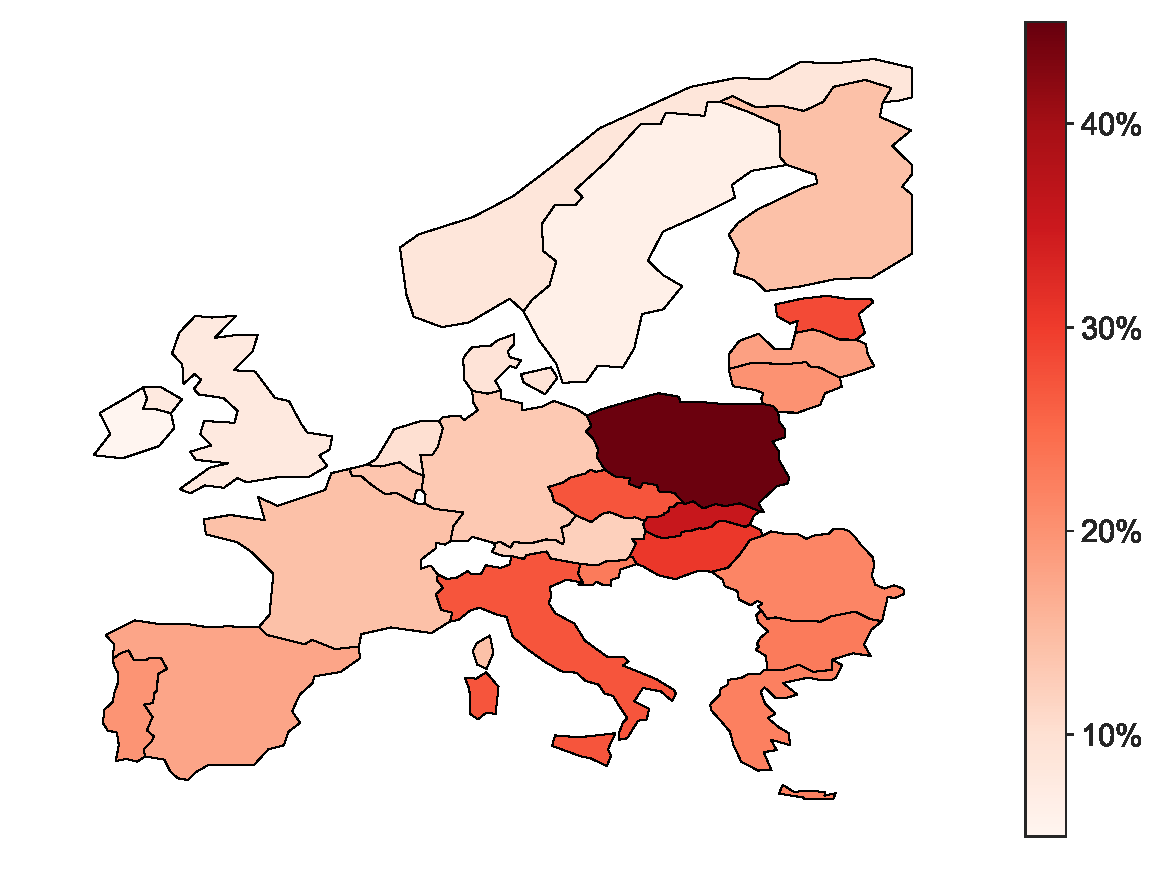
\includegraphics[width=.9\textwidth]{images/ted_networks/eu_sb_map.pdf}
\caption[Single bidding rates of EU countries.]{Single bidding rates of EU countries, 2008-2016.}
\label{fig:eu_sb_rates}
\end{figure*}


How does this measure correlate with the previously discussed survey-based measures of corruption risk? We find that national single bidding rates correlate significantly with a variety of corruption indicators discussed above, ranging in absolute value from .65 to .72.

\begin{figure*}[!ht]
\centering
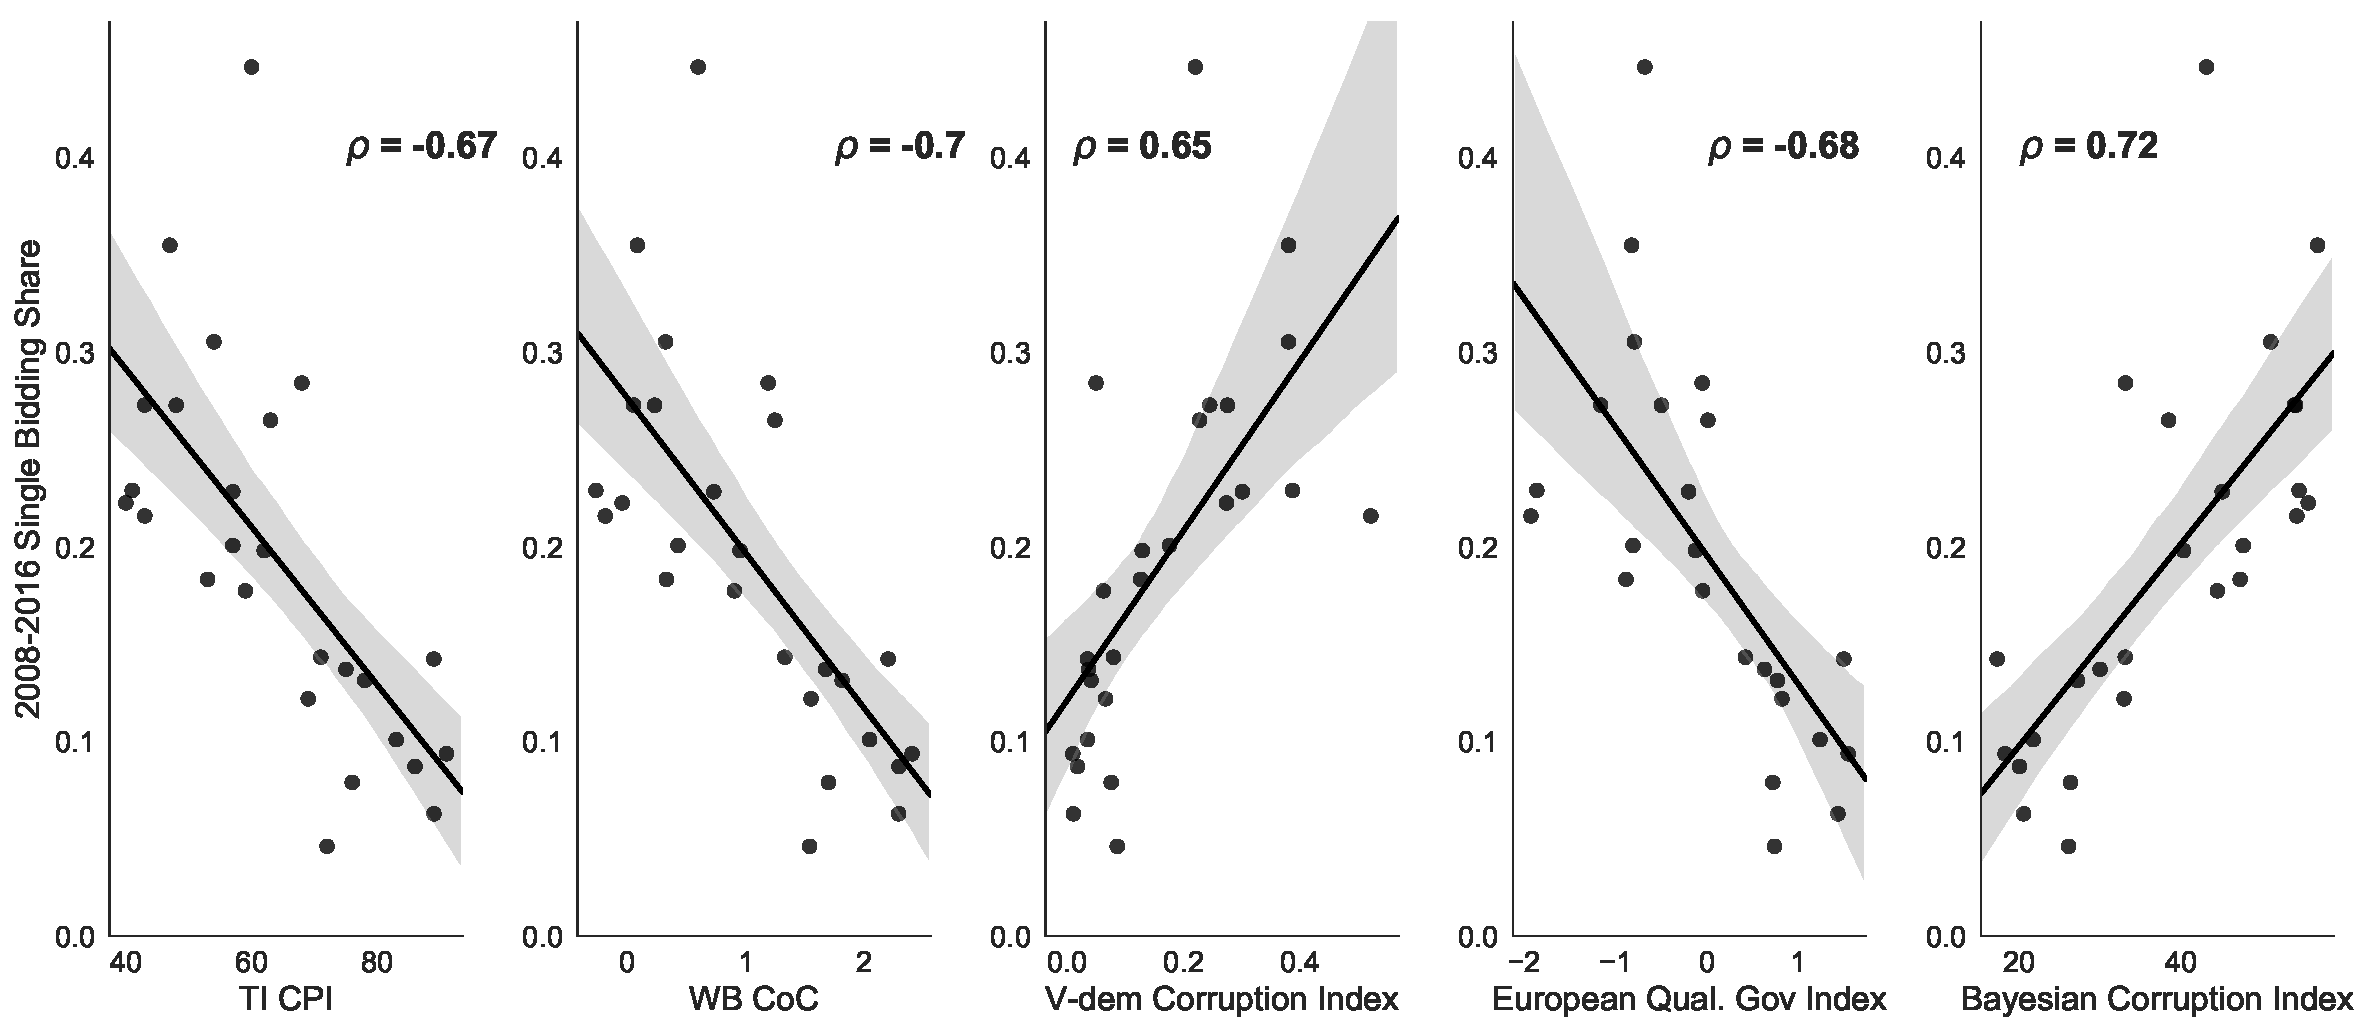
\includegraphics[width=\textwidth]{images/ted_networks/sb_corruption_correlations.pdf}
\caption[Correlates of national single bidding]{Correlation of national-level single bidding rates 2008-2016 with other commonly used measures of corruption in 2013. Where the correlation between the single bidding rate and the corruption indicator is negative the corruption indicator measures control of corruption and higher values indicate better outcomes.}
\label{fig:ted_sb_corr}
\end{figure*}


We will return to the national-level data in Chapter 4, in which we apply network science methods to describe the distribution of corruption risk in public procurement markets.

\section{Corruption as Networked Phenomenon}
We now turn our attention to past work on corruption, or criminal behavior more general, which employs network methods or perspective. Though we have mentioned network-based interpretations of the findings of related work in the previous sections, the works that we discuss now take an explicit network or relational approach to the study of corruption.

Many studies of organized crime, for instance the mafia represent the structure of the organization as a network~\cite{gambetta1996sicilian,calderoni2011strategic}, especially when transnational organizations are studied~\cite{williams2001transnational}. Network structure of contacts and command hierarchy reveal how these organizations function, how they structure themselves to be resilient to turncoats or attacks from rival organizations~\cite{agreste2016network,dellaposta2017network}. Similarly, networks provide a valuable perspective on the operation of terrorist cells~\cite{krebs2002mapping}.

White collar crime has also been studied using network methods. In an example from Canada, the diffuse network of actors responsible for various accounting procedures facilitated a significant corruption ring involving top members of a major political party~\cite{neu2013accounting}. Researchers have used email data from Enron, a major US Fortune 500 company which filed for bankruptcy in 2001 amid allegations of fraud and criminal conspiracy by its executives, to study patterns of communication during a crisis and criminal cover-up~\cite{diesner2005communication}.

In a more recent article, Ribeiro et al. investigated the temporal evolution of the network of co-conspirators in Brazilian political scandals over a 27 year period~\cite{ribeiro2018dynamical}. By the time of the Petrobras scandal, a giant connected component had emerged in the network of co-conspiracy, connecting a large majority of individuals. More broadly, network methods have been used to understand the co-occurrence of different sorts of criminality~\cite{tumminello2013phenomenology,rostami2015complexity}. For example, criminals often specialize in certain kinds of crimes (for instance financial crimes such as fraud) and tend to carry out new kinds of crime with accomplices who already have some experience. 
